% Created 2017-05-31 Wed 22:06
% -*- latex-run-command: pdflatex -*-
\documentclass[11pt]{article}
\usepackage[utf8]{inputenc}
\usepackage[T1]{fontenc}
\usepackage{graphicx}
\usepackage{grffile}
\usepackage{longtable}
\usepackage{wrapfig}
\usepackage{rotating}
\usepackage[normalem]{ulem}
\usepackage{amsmath}
\usepackage{textcomp}
\usepackage{amssymb}
\usepackage{capt-of}
\usepackage{hyperref}
\usepackage[margin=1.2in]{geometry}
\usepackage{setspace}
\singlespacing
\usepackage{parskip}
\usepackage[round]{natbib}
\setcounter{secnumdepth}{1}
\author{Zheng Tian}
\date{}
\title{The Application of California School}
\hypersetup{
 pdfauthor={Zheng Tian},
 pdftitle={The Application of California School},
 pdfkeywords={},
 pdfsubject={},
 pdfcreator={Emacs 25.1.1 (Org mode 9.0.7)},
 pdflang={English}}
\begin{document}

\maketitle


\section{Introduction}
\label{sec:org351368d}
This tutorial is to show how to estimate a multiple regression model
and perform linear hypothesis testing. The application is about the
test scores of the California school districts. We will use R to
replicate the multiple regression with this data set in Chapter 6, and
the hypothesis tests in Chapter 7, \citet{StockWatson2011}.

Before running all R codes, we may first load all the packages.
\begin{verbatim}
library(AER)
library(foreign)
library(stargazer)
\end{verbatim}


\section{Reading the data and basic summary statistics}
\label{sec:orgc71fbb1}
Let's first read the data into R and show some basic statistics.
\subsection*{Read the STATA file}
\label{sec:org0c0539c}
Since the data is stored as an STATA file with the extension
"\texttt{.dta}", we read the data using \texttt{read.dta()} in the library of
\texttt{foreign}.

\begin{verbatim}
setwd("/Users/ztian/OneDrive/teaching/workshop/intro_org_RR/example")
classdata <- read.dta("./data/caschool.dta")
\end{verbatim}

\subsection*{Summary}
\label{sec:orgfd9b14f}
Upon reading the data, we often use \texttt{summary()} to see some basic
statistics. Here we are not going to show summary statistics of all
variables in the data set for the purpose of saving space, but only to
select several variables of interest in Chapters 6 and 7, including
test scores, \texttt{testscr}, student-teacher ratio, \texttt{str}, percentage of
English learners, \texttt{el\_pct}, expenditure per pupil, \texttt{expn\_stu}, and
percentage of students qualifying for free lunch, \texttt{mean\_pct}.

\begin{verbatim}
summary(classdata[c("testscr", "str", "el_pct", "expn_stu", "meal_pct")])
\end{verbatim}

\begin{center}
\begin{tabular}{lllll}
testscr & str & el\_pct & expn\_stu & meal\_pct\\
\hline
Min.   :605.5 & Min.   :14.00 & Min.   : 0.000 & Min.   :3926 & Min.   :  0.00\\
1st Qu.:640.0 & 1st Qu.:18.58 & 1st Qu.: 1.941 & 1st Qu.:4906 & 1st Qu.: 23.28\\
Median :654.5 & Median :19.72 & Median : 8.778 & Median :5215 & Median : 41.75\\
Mean   :654.2 & Mean   :19.64 & Mean   :15.768 & Mean   :5312 & Mean   : 44.71\\
3rd Qu.:666.7 & 3rd Qu.:20.87 & 3rd Qu.:22.970 & 3rd Qu.:5601 & 3rd Qu.: 66.86\\
Max.   :706.8 & Max.   :25.80 & Max.   :85.540 & Max.   :7712 & Max.   :100.00\\
\end{tabular}
\end{center}


\section{Plots}
\label{sec:org41326aa}
\subsection*{Create a matrix of scatterplots using \texttt{plot}}
\label{sec:orge6d89e7}
We can create several scatterplots displayed in one graph with a
matrix form.

\begin{verbatim}
oldpar <- par(mfrow = c(2, 3))

plot(classdata$str, classdata$testscr, col = "red",
     main = "Student-teacher ratio vs test scores",
     xlab = "Student-teacher ratio", ylab = "Test scores")

plot(classdata$el_pct, classdata$testscr, col = "blue",
     main = "English learners vs test scores",
     xlab = "Percentage of English learners",
     ylab = "Test scores")

plot(classdata$expn_stu, classdata$testscr, col = "green3",
     main = "Expenditure per pupil vs test scores",
     xlab = "Expenditure per pupil",
     ylab = "Test scores")

plot(classdata$meal_pct, classdata$testscr, col = "maroon",
     main = "Free lunch vs test scores",
     xlab = "Percentage of students with free lunch",
     ylab = "Test scores")

plot(classdata$calw_pct, classdata$testscr, col = "darkorange1",
    main = "Public assistance vs test scores",
    xlab = "Percentage of students in public assistance",
    ylab = "Test scores")

par(oldpar)
\end{verbatim}

\begin{figure}[htbp]
\centering
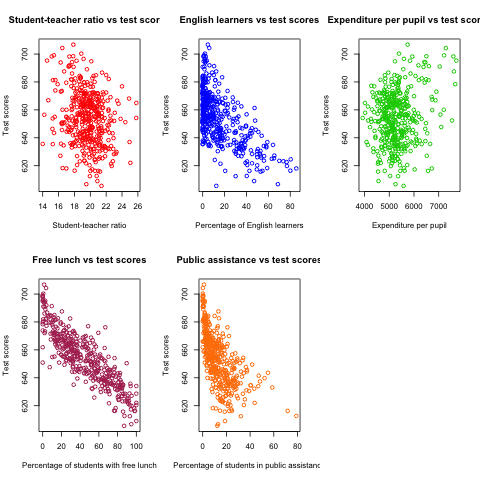
\includegraphics[width=0.7\textwidth,height=0.5\textheight]{./scplotmat.png}
\caption{The scatterplots between several variables and test scores}
\end{figure}


We can see that the codes above have some parts that are repeated in
each plotting command. So these repetitive work can be concisely
written in \texttt{for} a loop. The basic syntax of a \texttt{for} loop is
\texttt{for (var in seq) expr}.

\begin{verbatim}
xvars <- c("str", "el_pct", "expn_stu", "meal_pct", "calw_pct")
yvars <- c("testscr")

xlabels <- c("Student-teacher ratio", "Percentage of English learners",
             "Expenditure per pupil", "Percentage of students with free lunch",
             "Percentage of students in the public assistant program")
ylabels <- "Test scores"

titles <- c("student-teacher ratio vs test scores",
            "English learners vs test scores",
            "Expenditure per pupil vs test scores",
            "Free lunch vs test scores vs test scores",
            "public assistance vs test scores")
colors <- c("red", "green3", "blue", "maroon", "darkorange1")


op <- par(mfrow = c(2, 3))
for (i in seq(along=xvars)) {
    fm <- formula(paste(yvars, "~", xvars[i]))
    plot(fm, data = classdata, col = colors[i], main = titles[i],
         xlab = xlabels[i], ylab = ylabels)
}
par(op)
\end{verbatim}


\section{Estimation}
\label{sec:org55b9542}
Let us first replicate the regression results in Equation (7.19). The
unit of the expenditure per pupil is dollars in the data set but it is
in thousand dollars in regression. So we need to convert the unit in
the data set by dividing \texttt{expn\_stu} by 1000, which is done directly in
the formula.
\subsection*{The OLS estimation}
\label{sec:org3752626}

\begin{verbatim}
model.76 <- testscr ~ str + I(expn_stu / 1000) + el_pct
\end{verbatim}

Notice the function \texttt{I()} in the formula. The arithmetic operations,
+, *, :, /, and \^{}, have special meanings in R's formula. Using the
function \texttt{I()} protects the original arithmetic meanings of these
operations from being interpreted in terms of a formula.

The regression estimation can be done with \texttt{lm()} and use \texttt{summary()}
afterwards.

\begin{verbatim}
res.model.76 <- lm(model.76, data = classdata)
summary(res.model.76)
\end{verbatim}

\begin{verbatim}

Call:
lm(formula = model.76, data = classdata)

Residuals:
    Min      1Q  Median      3Q     Max
-51.340 -10.111   0.293  10.318  43.181

Coefficients:
                  Estimate Std. Error t value Pr(>|t|)
(Intercept)      649.57795   15.20572  42.719  < 2e-16 ***
str               -0.28640    0.48052  -0.596  0.55149
I(expn_stu/1000)   3.86790    1.41212   2.739  0.00643 **
el_pct            -0.65602    0.03911 -16.776  < 2e-16 ***
---
Signif. codes:  0 ‘***’ 0.001 ‘**’ 0.01 ‘*’ 0.05 ‘.’ 0.1 ‘ ’ 1

Residual standard error: 14.35 on 416 degrees of freedom
Multiple R-squared:  0.4366,	Adjusted R-squared:  0.4325
F-statistic: 107.5 on 3 and 416 DF,  p-value: < 2.2e-16
\end{verbatim}

We can extract some components in the reported results. Use \texttt{coef()} to
get the coefficient estimates, \texttt{resid()} to get the residuals, and \texttt{fitted()}
or \texttt{predict()} to get the fitted values. Alternatively, we can think the
\texttt{lm} and \texttt{summary.lm} objects returned by \texttt{lm()} and \texttt{summary()} are the
\texttt{list} object so that we can use the "\$" operator to get each component of
the lists. Below are some examples of extracting regression results.

\begin{verbatim}
# get some components of the results
bhat <- coef(res.model.76)
rsq <- summary(res.model.76)$r.squared
adj.rsq <- summary(res.model.76)$adj.r.squared
\end{verbatim}

\begin{itemize}
\item Interpretation of the results
\label{sec:org08474ce}

As for the coefficients
\begin{enumerate}
\item The intercept is \texttt{649.5779}, which is significant at
1\% significance level. It does not have real meaning in this
application, just determining the position of the sample regression
line crossing the vertical axis.
\item The coefficient on \texttt{str} is \texttt{-0.2864}, implying that
increasing one more student per teacher would decrease test scores
by \texttt{0.2864} unit. However, this estimated
coefficient is not significant at the 10\% level.
\item The coefficient on expenditure per pupil is \texttt{3.8679},
significantly positive at the 5\% level, implying that an increase in
expenditure per pupil by one thousand dollars lead to an increase
in test scores by \texttt{3.8679} unit.
\item The coefficient on the percentage of English learners is
\texttt{-0.656}, significantly negative at the 1\% level,
implying that an increase in the percentage of English learners by
one percent results in a decrease of test scores by
\texttt{0.656}.
\end{enumerate}

Besides, the \(R^2\) and \(\bar{R}^2\) are \texttt{0.4366} and
\texttt{0.4325}, respectively. Overall, the model explains
about 43\% variation of test scores with the included explanatory
variables, which is modest in the sense that a little more than half
of the variation of test scores is not accounted for in the model.
\end{itemize}

\subsection*{The heteroskedasticity-consistent covariance matrix}
\label{sec:org728e6c9}
Note that standard errors and t statisitcs reported by \texttt{summary()} are
the homoskedasticity-only s.e. and t's. The heteroskedasticity-robust
covariance matrix can be obtained by \texttt{vcovHC()} in the package of
\texttt{sandwich}.
\begin{verbatim}
htvarm <- vcovHC(res.model.76, type = "HC1")
\end{verbatim}

\begin{center}
\begin{tabular}{rrrr}
238.960380157595 & -6.66491920338914 & -20.7034584893236 & 0.0818068203778049\\
-6.66491920338933 & 0.232394197515306 & 0.40034628247013 & -0.00244872476838095\\
-20.7034584893232 & 0.400346282470112 & 2.49868335516912 & -0.0102366018665727\\
0.0818068203778026 & -0.00244872476838084 & -0.0102366018665727 & 0.00101024993508859\\
\end{tabular}
\end{center}


\section{Hypothesis tests}
\label{sec:org50e6906}
\subsection*{Testing a single coefficient}
\label{sec:org2a79d97}
Running \texttt{summary(res.model.76)} can give you t-statistics for all
coefficients. However, as noted above, these t-statistics are the
homoskedasticity-only t-statistics. We should use the
heteroskedasticity-robust ones.

\begin{verbatim}
# homoskedasticity-only
coeftest(res.model.76)

# heteroskedasticity-robust, t distribution
cftest.t <- coeftest(res.model.76, vcov = htvarm)
cftest.t

# heteroskedasticity-robust, normal distribution
cftest.n <- coeftest(res.model.76, vcov = htvarm, df = Inf)
cftest.n
\end{verbatim}

\begin{verbatim}
(Intercept)
   649.5779

   str
-0.2864

  str
0.2864
I(expn_stu/1000)
          3.8679
I(expn_stu/1000)
          3.8679
el_pct
-0.656
el_pct
 0.656
[1] 0.4366
[1] 0.4325

t test of coefficients:

                   Estimate Std. Error  t value  Pr(>|t|)
(Intercept)      649.577947  15.205719  42.7193 < 2.2e-16 ***
str               -0.286399   0.480523  -0.5960  0.551489
I(expn_stu/1000)   3.867902   1.412122   2.7391  0.006426 **
el_pct            -0.656023   0.039106 -16.7755 < 2.2e-16 ***
---
Signif. codes:  0 ‘***’ 0.001 ‘**’ 0.01 ‘*’ 0.05 ‘.’ 0.1 ‘ ’ 1

t test of coefficients:

                   Estimate Std. Error  t value Pr(>|t|)
(Intercept)      649.577947  15.458343  42.0212  < 2e-16 ***
str               -0.286399   0.482073  -0.5941  0.55277
I(expn_stu/1000)   3.867902   1.580722   2.4469  0.01482 *
el_pct            -0.656023   0.031784 -20.6397  < 2e-16 ***
---
Signif. codes:  0 ‘***’ 0.001 ‘**’ 0.01 ‘*’ 0.05 ‘.’ 0.1 ‘ ’ 1

z test of coefficients:

                   Estimate Std. Error  z value Pr(>|z|)
(Intercept)      649.577947  15.458343  42.0212  < 2e-16 ***
str               -0.286399   0.482073  -0.5941  0.55245
I(expn_stu/1000)   3.867902   1.580722   2.4469  0.01441 *
el_pct            -0.656023   0.031784 -20.6397  < 2e-16 ***
---
Signif. codes:  0 ‘***’ 0.001 ‘**’ 0.01 ‘*’ 0.05 ‘.’ 0.1 ‘ ’ 1
\end{verbatim}

We can see from the results above that
\begin{enumerate}
\item whether we use the homoskedasticity-only or
heteroskedasticity-robust variance matrices does not affect the
coefficient estimates because the calculation of these estimates
does not involve the variance matrices.
\item Using the homoskedasticity-only or
heteroskedasticity-robust variance matrices yields different
standard errors and t-statistics. Even though the
homoskedasticity-only standard errors of student-teacher ratios
seems smaller than the heteroskedasticity-robust ones, we cannot
say that the estimates with the homoskedasticity-only standard
errors are more efficient or precise because we are using a wrong
variance matrix in this case.
\item The p-values from t distribution and standard normal distribution
are slightly different, given the corresponding t-statistics are
identical in the two cases.
\end{enumerate}
\subsection*{Testing joint hypotheses}
\label{sec:org2f44e2c}
\begin{itemize}
\item Zero restrictions
\label{sec:orga911415}
Let's first test the joint zero restrictions.
\[ H_0:\, \beta_1 = 0, \beta_2 = 0 \text{ vs. } H_1: \beta_1 \neq 0
\text{ or } \beta_2 \neq 0 \]

We can use the function \texttt{linearHypothesis()} to test this and any linear
hypotheses.

\begin{verbatim}
test1 <- linearHypothesis(res.model.76,
	    c("str = 0", "I(expn_stu/1000) = 0"),
	    vcov = htvarm, test = "F")
test1
test1.F <- test1$F[2]
test1.p <- test1$"Pr(>F)"[2]
\end{verbatim}

\begin{verbatim}
Linear hypothesis test

Hypothesis:
str = 0
I(expn_stu/1000) = 0

Model 1: restricted model
Model 2: testscr ~ str + I(expn_stu/1000) + el_pct

Note: Coefficient covariance matrix supplied.

  Res.Df Df      F   Pr(>F)
1    418
2    416  2 5.4337 0.004682 **
---
Signif. codes:  0 ‘***’ 0.001 ‘**’ 0.01 ‘*’ 0.05 ‘.’ 0.1 ‘ ’ 1
\end{verbatim}

The F-statistic is \texttt{5.4337} with the p-value as
\texttt{0.0047}, which is less than 1\%. Therefore, we can
reject the null hypothesis at the 1\% level.

Note that the F-statistic is computed with the heteroskedasticity-robust
variance matrix and tested against a F distribution of (2, 416) degree
of freedom.

\item linear restrictions
\label{sec:org2ae458d}
Let's test the following restriction,
\[ H_0:\, \beta_1 + \beta_2 = 0, H_1: \beta_1 + \beta_2 \neq 0 \]

We still use \texttt{linearHypothesis()}. But this time we use the argument
\texttt{white.adjust} for which we specify "hc1" and test against a Chi-squared
distribution with one degree of freedom. Therefore, what we get is a
Wald statistic.

\begin{verbatim}
# b1 + b2 = 0
test2 <- linearHypothesis(res.model.76,
	    c("str + I(expn_stu/1000) = 0"),
	    white.adjust = "hc1", test = "Chisq")
test2
test2.x <- test2$Chisq[2]
test2.p <- test2$"Pr(>Chisq)"[2]
\end{verbatim}

\begin{verbatim}
[1] 5.4337
[1] 0.0047
Linear hypothesis test

Hypothesis:
str  + I(expn_stu/1000) = 0

Model 1: restricted model
Model 2: testscr ~ str + I(expn_stu/1000) + el_pct

Note: Coefficient covariance matrix supplied.

  Res.Df Df  Chisq Pr(>Chisq)
1    417
2    416  1 3.6319    0.05668 .
---
Signif. codes:  0 ‘***’ 0.001 ‘**’ 0.01 ‘*’ 0.05 ‘.’ 0.1 ‘ ’ 1
\end{verbatim}

The Wald statistic is \texttt{3.6319} and the p-value is
\texttt{0.0567}, which is less than 10\% and greater than 5\%.
That means that the null hypothesis can be rejected at the 10\% level
but not at the 5\% level. This result implies that the effects of
hiring more teachers on test scores could be to some extent similar to
increasing more expenditure per pupil.

The homoskedasticity-only F statistic can be computed without specifying
\texttt{vcov} or \texttt{white.adjust}.

\begin{verbatim}
# homoskedasticity-only F
test2.hm <- linearHypothesis(res.model.76,
	    c("str + I(expn_stu/1000) = 0"),
	    test = "F")
test2.hm
\end{verbatim}

\begin{verbatim}
[1] 3.6319
[1] 0.0567
Linear hypothesis test

Hypothesis:
str  + I(expn_stu/1000) = 0

Model 1: restricted model
Model 2: testscr ~ str + I(expn_stu/1000) + el_pct

  Res.Df   RSS Df Sum of Sq      F  Pr(>F)
1    417 86562
2    416 85700  1    862.09 4.1847 0.04142 *
---
Signif. codes:  0 ‘***’ 0.001 ‘**’ 0.01 ‘*’ 0.05 ‘.’ 0.1 ‘ ’ 1
\end{verbatim}

The homoskedasticity-only F test points to rejecting the null hypothesis
at both 5\% and 10\% levels.
\end{itemize}


\section{Control variables and model specifications}
\label{sec:org1c60775}
In this section we estimate different models for the application of
test scores. The variable of interest is student-teacher ratios,
\(STR\). In the base specification, we include the percentage of
students who are English learners, \(PctEL\), and the percentage of
students who are eligible for free or subsidized lunch, \(LchPct\), as
control variables. An alternative control variable is the percentage
of students who receive public assistance.

\begin{verbatim}
model1 <- lm(testscr ~ str, data = classdata)
model2 <- lm(testscr ~ str + el_pct, data = classdata)
model3 <- lm(testscr ~ str + el_pct + meal_pct, data = classdata)
model4 <- lm(testscr ~ str + el_pct + calw_pct, data = classdata)
model5 <- lm(testscr ~ str + el_pct + meal_pct + calw_pct, data = classdata)
\end{verbatim}

We compute the heteroskedasticity-robust standard errors for the
coefficients in all model specifications. The function \texttt{vcovHC} is
used to get the heteroskedasticity-consistent covariance matrix (HCCM), in
which we set the argument \texttt{type} to be \texttt{HC1}. The
heteroskedasticity-robust standard errors of coefficients are the
square roots of the diagonal elements of these HCCMs.

\begin{verbatim}
hccm1 <- vcovHC(model1, type = "HC1")
se1 <- sqrt(diag(hccm1))

hccm2 <- vcovHC(model2, type = "HC1")
se2 <- sqrt(diag(hccm2))

hccm3 <- vcovHC(model3, type = "HC1")
se3 <- sqrt(diag(hccm3))

hccm4 <- vcovHC(model4, type = "HC1")
se4 <- sqrt(diag(hccm4))

hccm5 <- vcovHC(model5, type = "HC1")
se5 <- sqrt(diag(hccm5))
\end{verbatim}

Finally, the results for all models are displayed in Table
(\ref{table:tbl71}) that replicates Table 7.1 in Chapter 7. To create
a \LaTeX{} table, we use the function \texttt{stargazer}.

\begin{verbatim}
stargazer(model1, model2, model3, model4, model5,
	  title = "Results of regressions of test scores and class size",
	  covariate.labels = c("student-teacher ratio",
			       "percent English learners",
			       "percent eligible for subsidized lunch",
			       "percent on public assistance"),
	  dep.var.caption = "average test scores in the district",
	  se = list(se1, se2, se3, se4, se5), df = FALSE,
	  font.size = "small",
	  header = FALSE,
	  label = "table:tbl71")
\end{verbatim}


\begin{table}[!htbp] \centering
  \caption{Results of regressions of test scores and class size}
  \label{table:tbl71}
\small
\begin{tabular}{@{\extracolsep{5pt}}lccccc}
\\[-1.8ex]\hline
\hline \\[-1.8ex]
 & \multicolumn{5}{c}{average test scores in the district} \\
\cline{2-6}
\\[-1.8ex] & \multicolumn{5}{c}{testscr} \\
\\[-1.8ex] & (1) & (2) & (3) & (4) & (5)\\
\hline \\[-1.8ex]
 student-teacher ratio & $-$2.280$^{***}$ & $-$1.101$^{**}$ & $-$0.998$^{***}$ & $-$1.308$^{***}$ & $-$1.014$^{***}$ \\
  & (0.519) & (0.433) & (0.270) & (0.339) & (0.269) \\
  & & & & & \\
 percent English learners &  & $-$0.650$^{***}$ & $-$0.122$^{***}$ & $-$0.488$^{***}$ & $-$0.130$^{***}$ \\
  &  & (0.031) & (0.033) & (0.030) & (0.036) \\
  & & & & & \\
 percent eligible for subsidized lunch &  &  & $-$0.547$^{***}$ &  & $-$0.529$^{***}$ \\
  &  &  & (0.024) &  & (0.038) \\
  & & & & & \\
 percent on public assistance &  &  &  & $-$0.790$^{***}$ & $-$0.048 \\
  &  &  &  & (0.068) & (0.059) \\
  & & & & & \\
 Constant & 698.933$^{***}$ & 686.032$^{***}$ & 700.150$^{***}$ & 697.999$^{***}$ & 700.392$^{***}$ \\
  & (10.364) & (8.728) & (5.568) & (6.920) & (5.537) \\
  & & & & & \\
\hline \\[-1.8ex]
Observations & 420 & 420 & 420 & 420 & 420 \\
R$^{2}$ & 0.051 & 0.426 & 0.775 & 0.629 & 0.775 \\
Adjusted R$^{2}$ & 0.049 & 0.424 & 0.773 & 0.626 & 0.773 \\
Residual Std. Error & 18.581 & 14.464 & 9.080 & 11.654 & 9.084 \\
F Statistic & 22.575$^{***}$ & 155.014$^{***}$ & 476.306$^{***}$ & 234.638$^{***}$ & 357.054$^{***}$ \\
\hline
\hline \\[-1.8ex]
\textit{Note:}  & \multicolumn{5}{r}{$^{*}$p$<$0.1; $^{**}$p$<$0.05; $^{***}$p$<$0.01} \\
\end{tabular}
\end{table}


\bibliography{example}
\bibliographystyle{plainnat}
\end{document}